\documentclass[a4paper,10pt, oneside]{article}
\usepackage[utf8]{inputenc}
\usepackage[spanish]{babel}
\usepackage[style=ieee,backend=bibtex]{biblatex}
\usepackage{graphicx}
\usepackage{lineno}
\usepackage[table]{xcolor}
%\usepackage{showframe}

\usepackage[top=1in, bottom=1.25in, left=1.25in, right=1.25in]{geometry}
\usepackage{caption}
\usepackage{bytefield}

\usepackage{lscape} 


\bibliography{informe_1}

	
\begin{document}
	
\begin{titlepage}
	\centering
	\includegraphics[width=0.25\textwidth]{../../Universidad_del_Litoral}\par\vspace{1cm}
	{\scshape\LARGE Universidad Nacional del Litoral \par}
	\vspace{1cm}
	{\scshape\Large Proyecto Final de Carrera\par}
	\vspace{1.5cm}
	{\huge\bfseries Diseño de un sistema de detección de anomalías en redes de computadoras.\par}
	\vspace{4cm}
	{\huge\bfseries Informe de avance 1\par}
	\vfill
	
	{\Large \itshape Pineda Leandro\par}
	
	
	% Bottom of the page
	\large Santa Fe\par
	{\large \today\par}	
\end{titlepage}

\modulolinenumbers[5]
\linenumbers


\section{Resumen}
El presente documento muestra los resultados obtenidos de la etapa de investigación del proyecto final de carrera de Ingeniería en Informática. En primer lugar dará una breve descripción de los distintos métodos existentes para la detección de anomalías. Luego se presentarán las técnicas de modelado a utilizar para detectar anomalías en el tráfico de red. Finalmente se describirán las tecnologías a utilizar, la arquitectura del sistema y sus componentes. 

\section{Detección de anomalías}
La detección de anomalías puede ser considerada como un problema de clasificación, donde comportamientos anómalos deben ser diferenciados de eventos normales\cite{baddar2014anomaly}. A continuación se describen los distintos enfoques analizados:
\subsection{Métodos de detección}
\subsubsection{Enfoque estadístico}
Este enfoque es usado cuando los comportamientos normales pueden ser ubicados en regiones de alta probabilidad de algún modelo estocástico, mientras que las anomalías pueden encontrarse en regiones de baja probabilidad de ese modelo\cite{Chandola:2009:ADS:1541880.1541882}. El modelo estocástico es determinado \textit{a priori} o es inferido a partir de un conjunto de datos. Bajo este enfoque, una anomalía es una observación que puede ser total o parcialmente irrelevante porque no está generada por un modelo estocástico dado. \par
Estos métodos de detección de anomalías ajustan un modelo estadístico (usualmente de comportamiento normal) a un conjunto de datos y luego, usando inferencia estadística, determinan si una nueva instancia pertenece a este modelo. Las instancias que tienen una baja probabilidad de ser generadas por el modelo ajustado son consideradas como anómalas.

\subsubsection{Enfoque espectral}
En algunas ocasiones muchas características de los patrones analizados son altamente independientes. Utilizar solo las dimensiones que son dependientes para describir los datos incrementa la precisión del modelo y reduce el costo computacional de los algoritmos. Matemáticamente, esta formulación es referida como reducción de dimensionalidades\cite{wang2012geometric}. Podemos pensar esta reducción como una representación de los datos en un espacio de menos dimensiones, de forma que instancias normales y anómalas se vean drásticamente diferentes. Una técnica popular de reducción de dimensionalidad es PCA (\textit{Principal Component Analysis}).

\subsubsection{Enfoque basado en Machine Learning}
En este enfoque se \textit{entrena} un algoritmo con datos de entrenamiento de forma que este ``aprenda'' cómo debería ser un comportamiento normal en el tráfico de red. Así, las anomalías son identificadas en base a la experiencia previa. Un algoritmo de \textit{machine learning} ``aprende'' una función que mapea todos las instancias de datos con alguno de los dos estados (usualmente representados con 0 y 1). \par

De acuerdo con la caracterización realizada en \cite{Chandola:2009:ADS:1541880.1541882}, podemos diferenciar los siguientes tipos de algoritmos basados en \textit{machine learning}:
\begin{itemize}
	\item \textbf{Basados en clasificación:} El objetivo de estos algoritmos es asignar cada dato a una clase (en este caso normal/anómalo), basandose en la información provista por un conjunto de características.
	\item \textbf{Algoritmos de vecino más cercano\footnote{En la literatura se encuentra como \textit{nearest-neighbor}}:} Estos algoritmos usan diferentes funciones (basadas en alguna métrica como distancia o densidad) para medir la diferencia entre una instancia de los datos y su \textit{k-ésimo} vecino más cercano\cite{Chandola:2009:ADS:1541880.1541882}. Esta diferencia o distancia es un puntaje que puede ser utilizado para decidir si la instancia es o no una anomalía.
	\item \textbf{Clustering:} Estos algoritmos buscan en los datos de entrenamiento grupos de instancias muy similares o cercanas entre si. Las anomalías pueden formar grupos de muy pocos elementos o no pertenecer a ningún grupo. Mapas auto-organizativos\cite{Kohonen:1997:SM:261082} y algorítmos de k-medias\cite{Hartigan/Wong:79} son algoritmos clásicos de clustering.
\end{itemize}

\subsubsection{El enfoque de \textit{streaming}}
En muchos casos, detectar anomalías en una red significa llevar registro de cambios significativos en los patrones de tráfico de red, como número de flujos activos o volumen de tráfico actual. Esto hace que sea necesario aplicar técnicas de detección que sean escalables, puesto que en redes donde circulan grandes volúmenes de información, registrar estos cambios en cada flujo de tráfico puede ser una tarea con un gran costo computacional.
El enfoque de \textit{streaming} analiza flujos continuos de datos y extrae información de cada uno, utilizando algoritmos discretos para detectar anomalías\cite{Cormode:2010:ANG:1805876} y evitar así tomar muestras del tráfico cada cierto tiempo, práctica típicamente utilizada en los algoritmos de detección de anomalías para solucionar el problema de la escalabilidad. Sin embargo, atacar el problema de la escalabilidad con muestreo involucra una disminución en la precisión de los sistemas de detección de anomalías ya que los paquetes que no son tenidos en cuenta pueden contener información importante para determinar la existencia de tales eventos.

\subsection{Comparación de los métodos}
Los métodos supervisados (sin importar que enfoque utilicen) necesitan de grandes \textit{dataset} de comportamiento normal o un conjunto de datos anómalos conocidos e identificados. Construir un modelo basado en una base de datos hace que calidad de las clasificaciones realizadas por el mismo dependa directamente de la calidad de los datos: un modelo no puede ser mejor que el \textit{dataset} con el cual se lo construyó. Más aún, la implementación en diferentes ámbitos de producción hace necesario que el modelo sea recalculado para un conjunto de datos que son propios de la infraestructura de red los cuales, en general, no están disponibles.\par
Una desventaja de los métodos basados en modelos estadísticos es que pueden ser ``entrenados'' gradualmente de forma que el tráfico generado durante un ataque se identificado como normal. Además, la puesta en funcionamiento de este tipo de sistemas toma períodos largos de tiempo dado que la construcción de los modelos estocásticos involucra analizar grandes volumenes de datos. Por otro lado, los modelos no requieren conocimiento previo ya que tiene la habilidad de ``aprender'' el comportamiento esperado procesando los datos del tráfico de red\cite{journals/comsur/BhuyanBK14}.\par
Los enfoques de clustering y vecindad utilizan métodos no supervisados. Aunque esto es una gran ventaja con respecto a los \textit{dataset}, su precisión es muy dependiente de las métricas utilizadas: el uso de una medida poco adecuada de proximidad afecta negativamente la capacidad de detección de los algoritmos de vecindad.\par
Las técnicas \textit{on-line}\footnotetext{término que refiere a los algoritmos que procesan la información del tráfico de red mientras se genera, opuesto a los algoritmos \textit{batch}} generalmente muestrean los datos para reducir la carga computacional de los algoritmos, descartando información que puede ser importante para que el sistema clasifique adecuadamente un evento. En los últimos años, las arquitecturas de \textit{streaming} distribuido (por ejemplo Flume\cite{apacheflume}, Apache Storm\cite{apachestorm} y Spark Streaming\cite{apachespark}) permitieron desarrollar algoritmos que aprovechen la capacidad de cálculo paralelo para mejorar la eficiencia en la clasificación y solucionar el problema de la escalabilidad\cite{huang2014ld}. La ventaja más importante de estas técnicas es la posibilidad de realizar las tareas de detección en forma distribuida: esto permite combinar múltiples resultados de detección de forma de reducir la cantidad de falsos positivos, aspecto de gran importancia en los sistemas de detección de anomalías y que además permite escalabilidad. Este último aspecto es también de gran importancia: la reciente aparición de ataques distribuidos masivos\footnote{https://krebsonsecurity.com/2016/09/krebsonsecurity-hit-with-record-ddos/} hace que sea necesario pensar el diseño de los nuevos sistemas de detección de anomalías para que funcionen en arquitecturas escalables y tolerante a fallas.

\section{Método de detección propuesto}
El tráfico de red puede ser caracterizado por la información disponible en la cabecera de los paquetes. El modelo TCP/IP establece que los host deben soportar como mínimo los protocolos IP, ICMP, TCP y UDP\cite{rfc1122}. Estos tienen en común una dirección de origen y destino: en capa de red se utilizan direcciones IP\cite{rfc791} y en capa de transporte se utilizan puertos\cite{rfc768}\cite{rfc793}. \par

Podemos identificar entonces un flujo de datos entre dos \textit{host} por una tupla de 5 valores (en adelante se hará referencia a estas tuplas como \textit{keys}). Estas \textit{keys} forman un espacio de $2^{104}$ características\footnote{Cada dirección IP es de 32 bits, cada puerto de 16 bits y el protocolo es un valor de 8 bits}:
\[\langle IP\ de\ origen,\ IP\ de\ destino,\ puerto\ de\ origen,\ puerto\ de\ destino,\ protocolo \rangle\]
Caracterizar tráfico normal en tiempo real utilizando un espacio de tantas dimensiones implica el uso de grandes cantidades de memoria. Más aún, las plataformas convencionales que utilizan sistemas de un solo procesador no proveen suficiente poder de cómputo para procesar cantidades masivas de flujos de datos en espacios de altas dimensionalidades. \par
Las técnicas basadas en conteo y las técnicas de basadas en \textit{sketch}\cite{krishnamurthy2003sketch}\cite{muthukrishnan2005data} pueden implementarse usando estructuras de datos eficientes para detectar anomalías en grandes espacios de características\cite{huang2014ld}. La primera técnica utiliza contadores que son actualizados a medida que se procesan nuevas tuplas. La segunda utiliza \textit{sketchs}: son matrices que permiten representar un gran conjunto de datos como otro conjunto de datos de menor tamaño. Un buen \textit{sketch} de un \textit{dataset} es aquel que puede utilizarse en lugar del \textit{dataset} en un cálculo, sin perder mucha precisión\cite{liberty2013simple}.
\par
Las anomalías, llamadas \textit{heavy keys}, pueden identificarse formulando el problema de detección en dos partes: detección de \textit{heavy hitter} y detección de \textit{heavy change}. El objetivo de la detección de \textit{heavy hitter} es identificar el conjunto de flujos o \textit{keys} que representan la mayor porción del tráfico de red o la capacidad del canal de comunicación\cite{estan2002new}. Por otro lado, en el problema de detección de \textit{heavy change}, el objetivo es detectar el conjunto de \textit{keys} que tienen cambios abruptos en el volumen de tráfico que transportan, entre un período de tiempo y el próximo\cite{krishnamurthy2003sketch}. La detección de \textit{heavy keys} puede realizarse mediante las técnicas de conteo y \textit{sketch}, procesando \textit{streams} de datos en tiempo real en un espacio sublineal en N. Además, el algoritmo es perfectamente paralelizable\cite{liberty2013simple}. Más aún, las lecturas y actualizaciones a los valores del \textit{sketch} son muy eficientes y pueden hacerse en tiempo constante\cite{goyal2010sketching}.

\section{Arquitectura del sistema}
Los datos serán capturados utilizando la librería \textit{libpcap}\footnote{http://www.tcpdump.org/}. Luego, el \textit{stream} de datos es procesado usando las técnicas de conteo y \textit{sketch} mencionadas previamente para llenar las estructuras de datos necesarias. El módulo de detección de anomalías analiza las estructuras de datos calculadas y determina la presencia de \textit{heavy keys}. Estas son almacenadas en un archivo de log. Finalmente la interfaz web presenta la información de las \textit{keys} analizadas, las estadísticas del sistema y muestra las anomalías detectadas.

\begin{figure}[htpb]
	\centering
	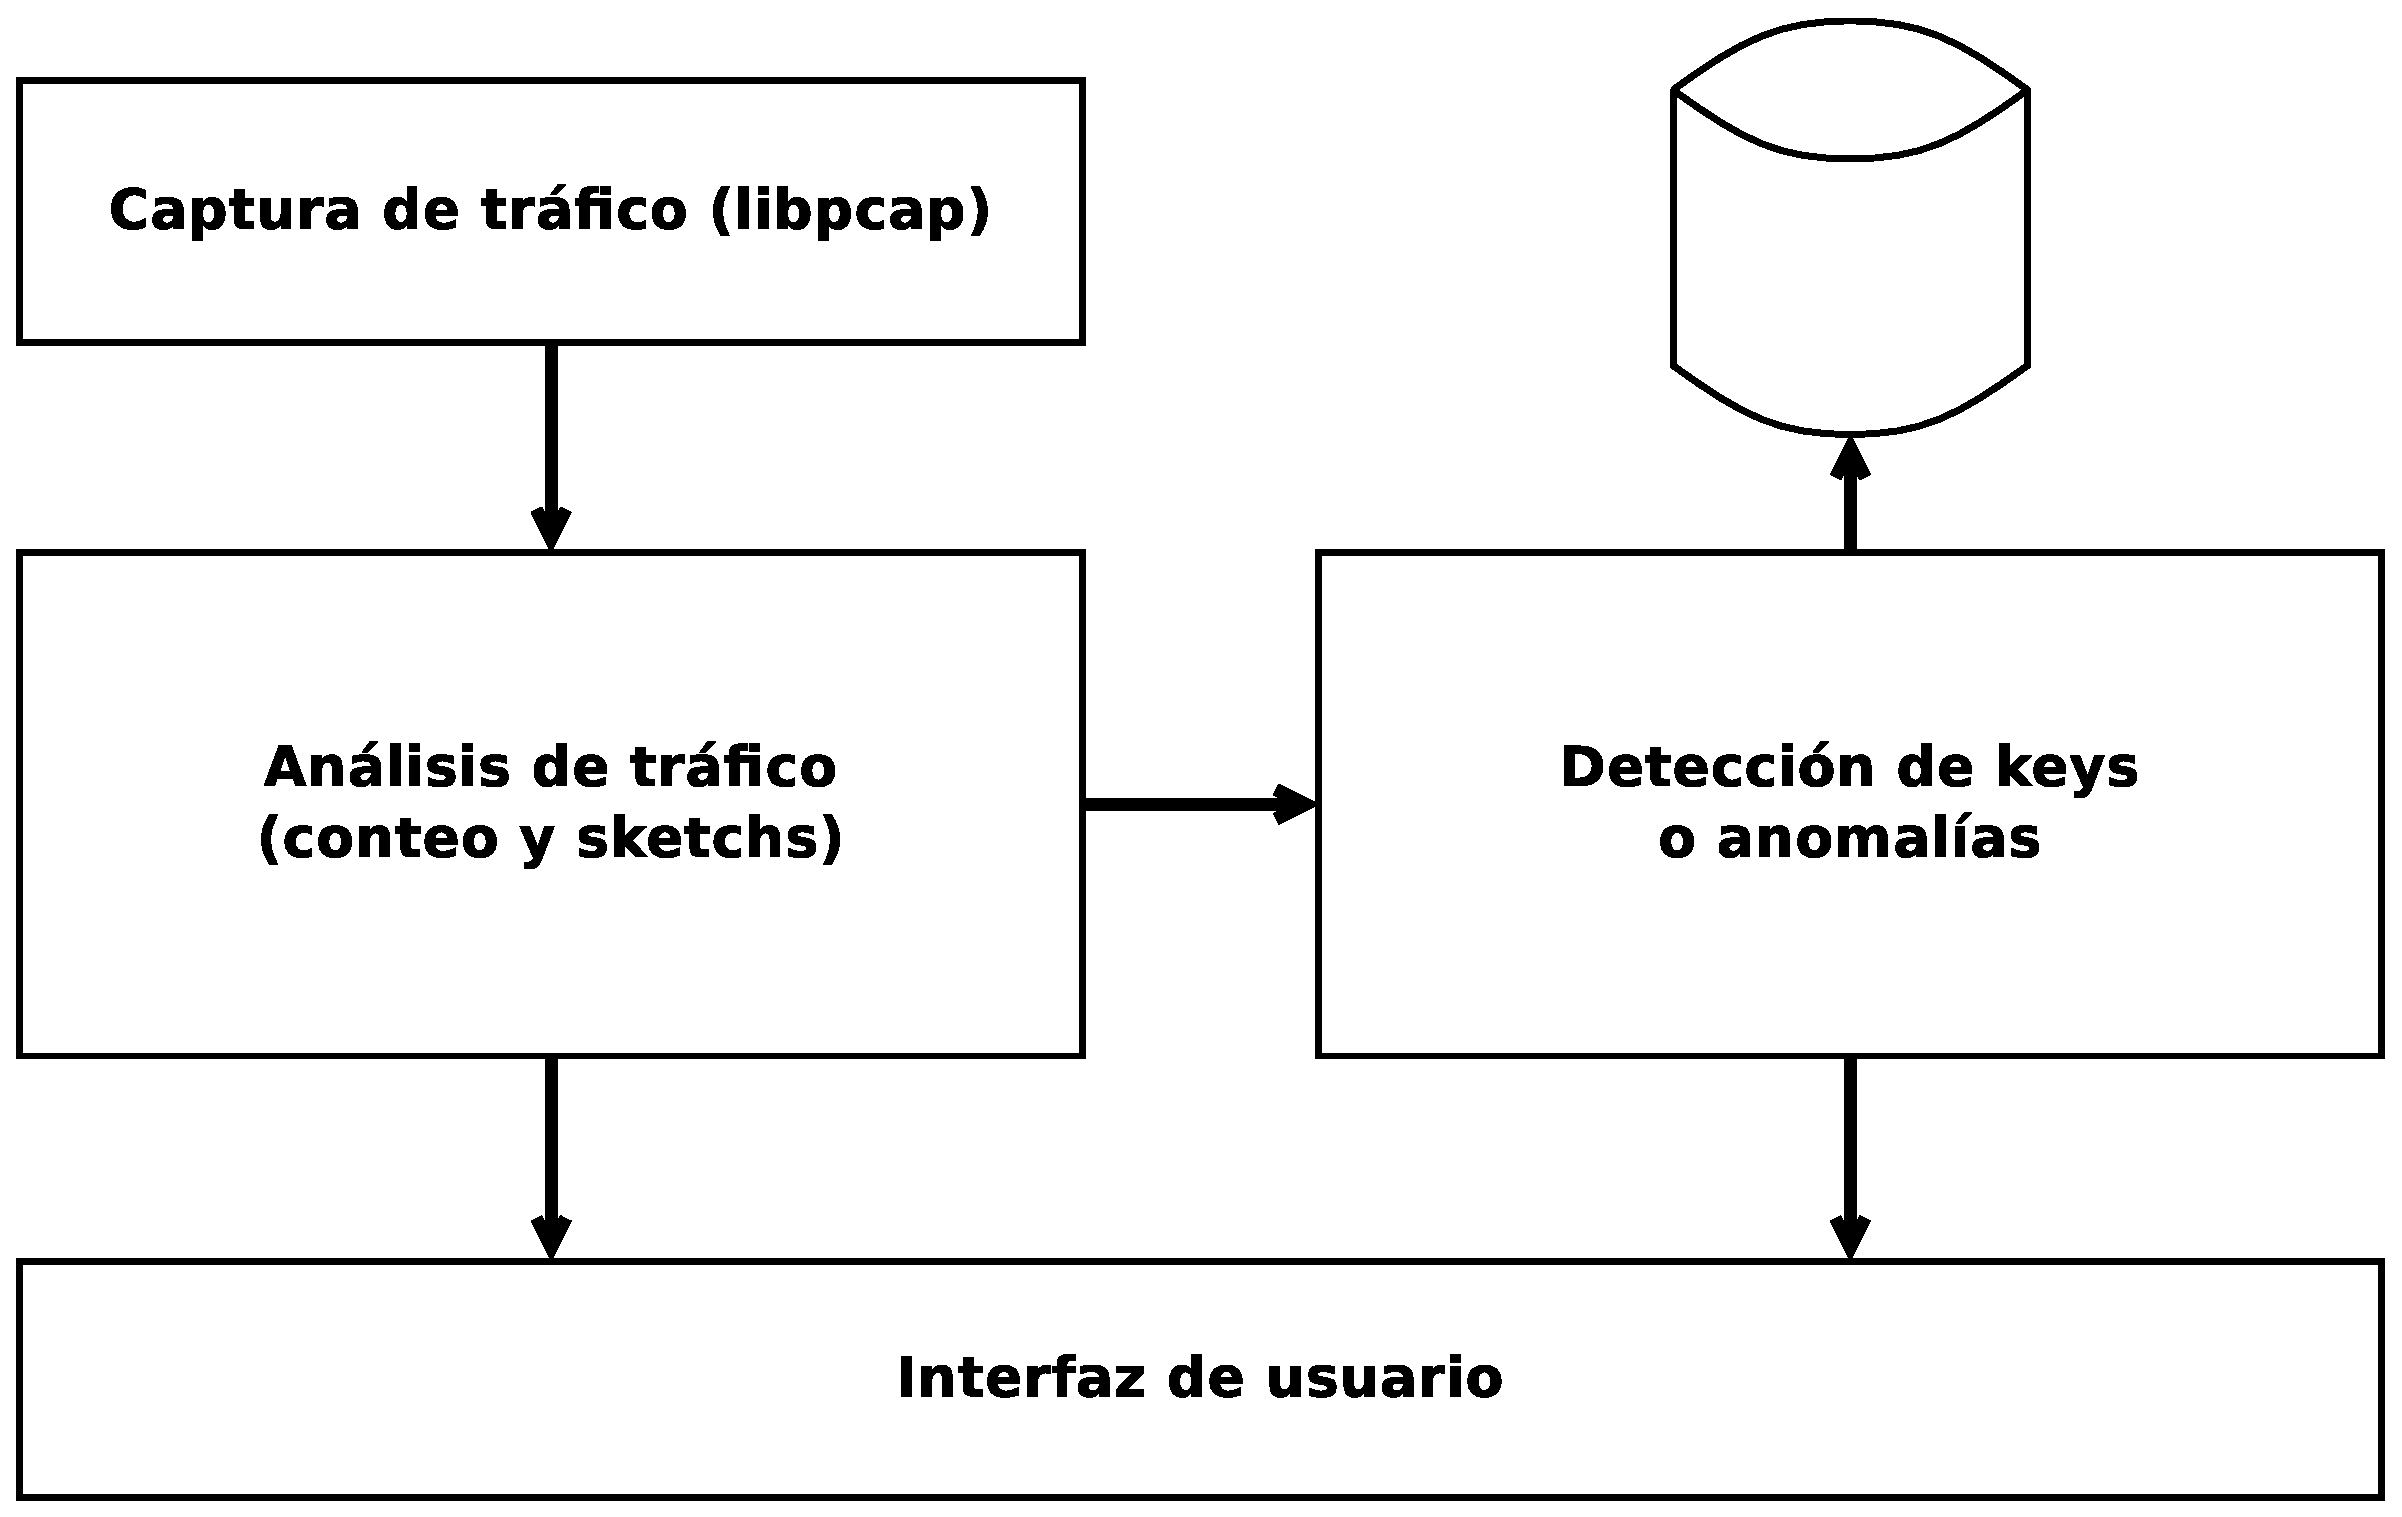
\includegraphics[scale=0.2]{graph/arquitectura}
	\caption{Arquitectura del sistema}
\end{figure}

\subsection*{Tecnologías a utilizar}
\subsubsection*{Data Streaming Frameworks}
Actualmente la comunidad de software libre mantiene tres frameworks importantes para procesamiento de \textit{streams} de datos. A continuación se da una descripción de cada uno:
\begin{itemize}
	\item Spark Streaming: es una extensión del API de Apache Spark, un sistema de propósito general para procesamiento de datos en \textit{cluster} de computadoras. Spark Streaming permite construir modelos de procesamiento de \textit{streams} de datos de manera escalable, con garantía de que los datos serán procesados una y solo una vez, tolerante a fallos y de alto desempeño. Incorpora también funciones de alto nivel como \textit{map}, \textit{reduce}, \textit{join} y \textit{window}. Spark Streaming no procesa estrictamente los datos en tiempo real sino que procesa pequeños lotes o \textit{mini-batches} a intervalos de tiempo dados.
	\item Apache Storm: es un sistema de cálculo distribuido en tiempo real. Los \textit{streams} de datos son analizados como eventos en lugar de una serie de \textit{mini-batches}. Esto significa que Storm tiene muy baja latencia y es ideal para datos que deben ser procesados como una sola entidad. Es escalable, tolerante a fallas, garantiza que los datos serán procesados al menos una vez.\par
	Apache Storm fue diseñado para ser utilizado con cualquier lenguaje de programación. Utiliza  \textit{Thrift}\footnote{http://thrift.apache.org/} para definir y ejecutar topologias por lo que las mismas pueden ser desarrolladas en cualquier lenguaje.
	\item Apache Flink: es una plataforma de código abierto para procesamiento distribuido de datos mediante \textit{batches} o \textit{streaming}. A diferencia de los dos anteriores, Flink asegura que los datos serán procesados una única vez sin agregar latencia como como ocurre con Spark Streaming. Además, el mecanismo que implementa para asegurar tolerancia a fallos distribuida es liviano\cite{chandy1985distributed}, lo que permite a la plataforma procesar grandes volúmenes de datos y mantener su consistencia.
	\par Flink únicamente soporta los lenguajes de programación Java y Scala. Esto debe ser así dado que implementa su propio espacio de memoria dentro de una máquina virtual Java, y debe ejecutar lenguajes compatibles.	
\end{itemize}

\begin{figure}[htpb]
	\centering
	\begin{tabular}{|l|l|l|l|}
		\hline
		& Spark Streaming & Storm & Flink \\
		\hline
		Procesamiento & \textit{micro-batching} & Tiempo real & Tiempo real \\
		Latencia & Alta & Baja & Baja \\
		Garantia de proceso & Exactamente una & Una o más & Exactamente una \\
		Lenguaje API & Python, Scala, Java & Multilenguaje & Scala, Java \\
		Procesamiento distribuido & Si & Si & Si \\
		\hline
	\end{tabular}
	\caption*{Resumen de las tecnologías analizadas}
\end{figure}

Dadas los \textit{framework} analizados, la selección adecuada para el desarrollo del proyecto es Apache Flink. En cualquier sistema de seguridad de información son necesarias tolerancia a fallos y alto desempeño.\par
Apache Storm ofrece alto desempeño, pero por su diseño asegura que las \textit{keys} serán procesadas al menos una vez, sin dar garantías de repeticiones en las tuplas. Por otro lado, Spark Streaming no es adecuado para la aplicación que se quiere desarrollar pues tiene bajo desempeño debido al uso de \textit{micro-batching}.

\newpage
\section*{Anexos}

\begin{figure}[htpb]
	\centering
	\begin{bytefield}{32}
		\bitheader{0,3,4,7,8,15,16,18,19,23,24,31} \\
		\bitbox{4}{Version} &
		\bitbox{4}{IHL} &
		\bitbox{8}{\small Type of Service} &
		\bitbox{16}{Total Length} \\
		\bitbox{16}{Identification} &
		\bitbox{3}{Flags} &
		\bitbox{13}{Fragment Offset} \\
		\bitbox{8}{Time to Live} &
		\bitbox{8}{Protocol} &
		\bitbox{16}{Header Checksum} \\
		\bitbox{32}{Source Address} \\
		\bitbox{32}{Destination Address} \\
		\bitbox{24}{Options} &
		\bitbox{8}{Padding} \\
	\end{bytefield}
	\caption{Cabecera IP}
	\vspace{1cm}
	
	\begin{bytefield}{32}
		\bitheader{0,7,8,15,16,31} \\
		\bitbox{8}{Type} &
		\bitbox{8}{Code} &
		\bitbox{16}{Checksum} \\
		\bitbox{32}{Rest of header} \\
		\wordbox{2}{Internet Header + 8 bytes of Original Datagram} \\
	\end{bytefield}
	\caption{Cabecera ICMP}
	\vspace{1cm}
	
	\begin{bytefield}{32}
		\bitheader{0,15,31} \\
		\bitbox{16}{Source Port} &
		\bitbox{16}{Destination Port} \\
		\bitbox{16}{Sequence Number} &
		\bitbox{16}{Acknowlegment Number} \\
	\end{bytefield}
	\caption{Cabecera UDP}
	\vspace{1cm}
				
	\begin{bytefield}{32}
		\bitheader{0,3,4,6,7,15,16,31} \\
		\bitbox{16}{Source Port} &
		\bitbox{16}{Destination Port} \\
		\bitbox{32}{Sequence Number} \\
		\bitbox{32}{Acknowlegment Number} \\
		\bitbox{4}{Offset} &
		\bitbox{3}{} &
		\bitbox{9}{Flags} &
		\bitbox{16}{Window Size} \\
		\bitbox{16}{Checksum} &
		\bitbox{16}{Urgent Pointer} \\
	\end{bytefield}
	\caption{Cabecera TCP}
\end{figure}



\newpage
\nocite{*}
\printbibliography
\end{document}

